\documentclass[14pt]{beamer}
\usetheme{Warsaw}
\usepackage[utf8]{inputenc}
\usepackage[german]{babel}
\usepackage[T1]{fontenc}
\usepackage{amsmath}
\usepackage{amsfonts}
\usepackage{amssymb}
\usepackage{graphicx}
%\author{}
%\title{}
%\setbeamercovered{transparent} 
%\setbeamertemplate{navigation symbols}{} 
%\logo{} 
%\institute{} 
%\date{} 
%\subject{} 
\begin{document}

%\begin{frame}
%\titlepage
%\end{frame}

%\begin{frame}
%\tableofcontents
%\end{frame}

\begin{frame}{Resonanzfrequenzen - Aufbau}
\begin{figure}
\begin{flushleft}
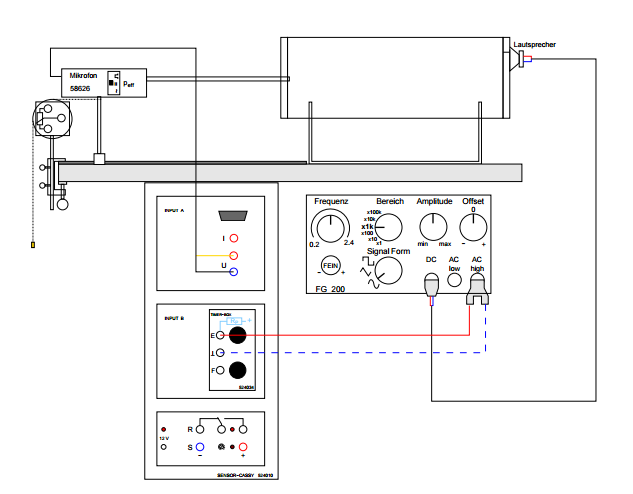
\includegraphics[scale=0.35]{aufbau}
\end{flushleft}
\end{figure}

\begin{flushright}
\begin{itemize}
\item  Messbereich Spannung: $0-3V$ ,Nullpunkt links, gemittelt über $1s$.
\item Timer-Box Bereich bis $5000Hz$, Torzeit $1s$
\item manuelle Messung
\end{itemize}
\end{flushright}
\end{frame}

\begin{frame}{Resonanzfrequenzen - Ergebnisse I}
\begin{figure}
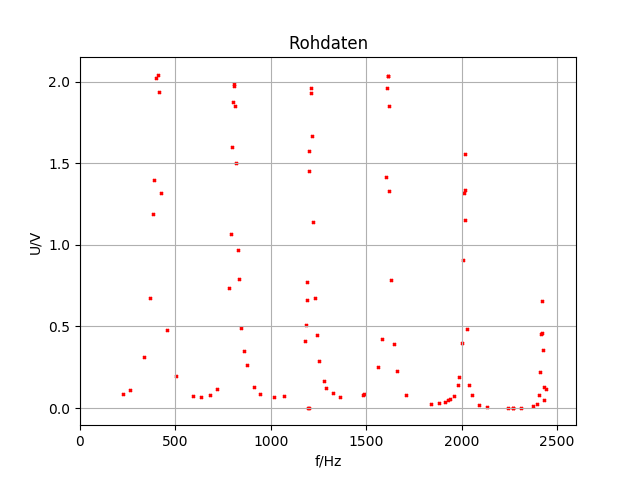
\includegraphics[scale=0.5]{rohres}
\end{figure}
\end{frame}

\begin{frame}{Resonanzfrequenzen - Ergebnisse II}
\begin{table}
\begin{tabular}{|c|c|c|}
\hline 
$n$ & $f[Hz]$ & $\sigma_f$ \\ 
\hline 
1 & 404.11 & 1.47 \\ 
\hline 
2 & 809.60 & 1.72 \\ 
\hline 
3 & 1209.22 & 1.29 \\ 
\hline 
4 & 1613.86 & 1.32 \\ 
\hline 
5 & 2013.32 & 1.29 \\ 
\hline 
6 & 2420.10 & 0.96 \\ 
\hline
\end{tabular} 
\end{table}
\end{frame}

\begin{frame}{Resonanzfrequenzen - Auswertung I}
\begin{figure}
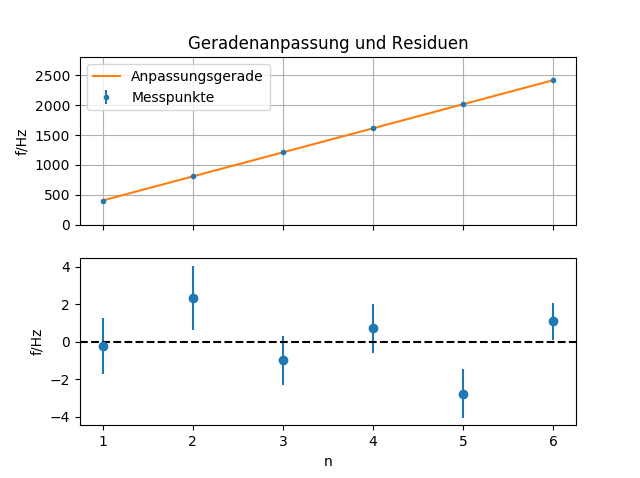
\includegraphics[width=\linewidth , height=0.75\textheight]{fitplot}
\end{figure}
\end{frame}

\begin{frame}{Resonanzfrequenzen - Auswertung II}
\begin{itemize}
\item Regression: $f(n)=a n+b$
\item $a=402.94Hz \quad \sigma_a=0.30Hz$
\item $b=1.40Hz \quad \sigma_b=1.32Hz$
\item $\chi^2/ndof=2.13$
\item $v=\lambda f = 344.91m/s$
\item $\Rightarrow \sigma_{v,stat.}=0.35m/s$
\item $\Rightarrow \sigma_{v,syst.}=0.56m/s$
\end{itemize}
\end{frame}

\begin{frame}{Druckverlauf - Aufbau}
\begin{itemize}
\item Aufbau weitesgehend identlisch zu Teilv. 1
\item $f=2017Hz$
\item Messbereich Spannung $0-3V$, Nullpunkt links und gemittelt über $100ms$.
\item Widerstandsbereich $0-3k \Omega$
\item Messparameter automatisch $100ms$.
\end{itemize}

\end{frame}

\begin{frame}{Druckverlauf - Ergebnisse}
\begin{figure}
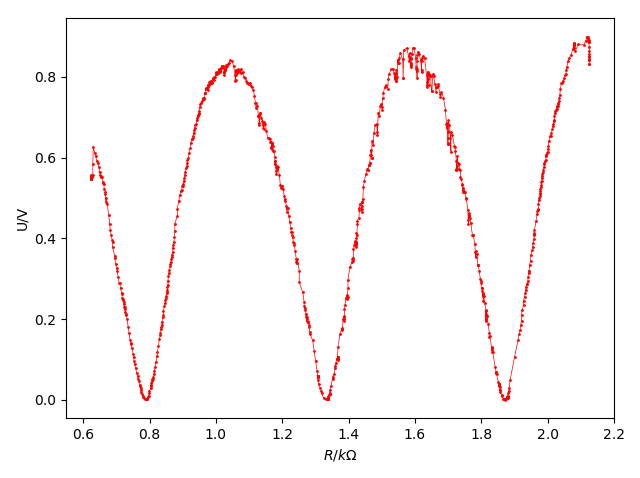
\includegraphics[scale=0.5]{druckverlauf}
\end{figure}
\end{frame}

\begin{frame}{Ergebnisse und Auswertung}
\begin{table}
\begin{tabular}{|c|c|c|}
\hline 
n & $R[k\Omega]$ & $\sigma_R[k\Omega]$ \\ 
\hline 
1 & 0.788 & 0.006 \\ 
\hline 
2 & 1.344 & 0.006 \\ 
\hline 
3 & 1.872 & 0.006 \\ 
\hline 
\end{tabular} 
\end{table}

\begin{figure}
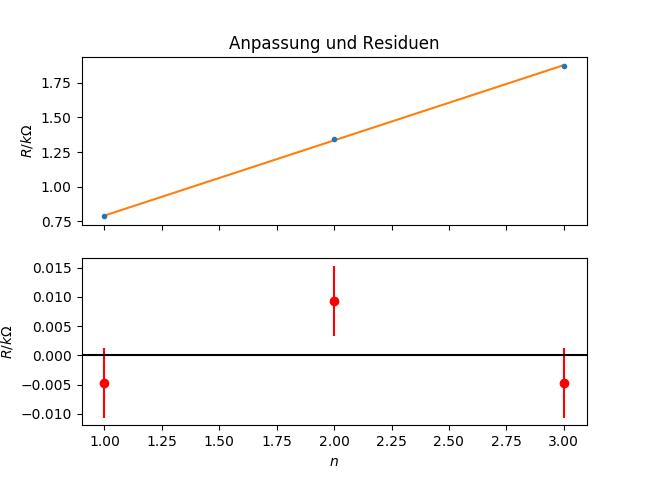
\includegraphics[scale=0.37]{fitdruckknoten}
\end{figure}
\end{frame}

\begin{frame}
\begin{itemize}
\item $R(n)=a \cdot n+b$
\item $a=0.542k\Omega \quad \sigma_{a}=0.004k\Omega$
\item $b=0.251k\Omega \quad \sigma_b=0.009k\Omega$
\item $\chi^2/ndof=3.630$
\item $\lambda=2Ka=17.31cm$
\item $f=2017.0Hz \quad \Rightarrow \quad v=f \lambda = 349.14m/s$
\item $\sigma_f=0.3Hz \quad \Rightarrow \sigma_{v,stat.}=2.63m/s$
\item $\sigma_{v,syst.}=f \sigma_{\lambda,syst.}=1.61m/s$
\end{itemize}
\end{frame}

\end{document}